\section{Results}
\subsection{RQ1: Coverage and Exposure Favor Different Selections}
Table~\ref{tab:methods} reports workflow-repository outcomes at 100 identities (0.819\% of usernames). Greedy covers \GreedyCovered{} repositories (\GreedyCoveragePercent{}\%), versus \UnionCovered{} (61.5\%) for exact union: a descriptive difference of $\Delta C = +1{,}131$ repositories (+25.7\%). Exact union instead removes \UnionExposurePercent{}\% of stipulated exposure, versus \GreedyExposurePercent{}\% for greedy ($\Delta H = -22.30$ percentage points; $\Delta P = +266$). Its $H$ advantage follows analytically; the experiment quantifies the resulting coverage tradeoff. Maximum reach nears this $H$ but covers fewer repositories.

\begin{table}[t]
\centering
\caption{Workflow-repository results at 100 identities. $C$: distinct coverage; $H$: conditional scenario exposure reduction; $P$: all-source exclusion. Random values are 200-order means.}
\label{tab:methods}
\small
\begin{tabular}{lrrrr}
\toprule
Selection & $C$ & $C$ (\%) & $H$ (\%) & $P$\\
\midrule
\ResearchMethodRows
\bottomrule
\end{tabular}
\end{table}

Figure~\ref{fig:budget} compares all six budgets. At 100, the 200 random orders give mean coverage 1,680.6 (sample SD 530.7; Monte Carlo standard error $\text{MCSE}_C=37.5$). Their mean $H$ is 0.80\% (SD 0.373 pp; $\text{MCSE}_H=0.026$ pp). The exact expectations are $E[C]=1{,}716.8$ and $E[H]=100/12{,}217=0.819\%$. These differences arise between finite random selections on the retained graph.



\subsection{RQ2: Covered Endpoints Retain Other Sources}
Figure~\ref{fig:sources} shows source multiplicities; Fig.~\ref{fig:partition} partitions source-reachable repositories at budget 100. Of the 5,538 repositories covered by greedy, only 800 meet all-source exclusion; 4,738 remain reachable from an unselected identity. Across the 7,158 repositories with nonempty observed source sets, 6,358 retain such a source. Exact-union ranking excludes every observed source for 534 repositories. Neither baseline optimizes $P$.

\begin{figure}[t]
\centering
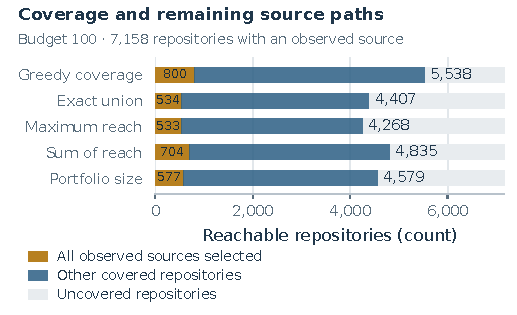
\includegraphics[width=\columnwidth]{coverage_partition.pdf}
\caption{Repository source-set partition at budget 100. Segment labels give all-source exclusion, covered residual exposure, and uncovered counts. Bars exclude 13 repositories without observed sources. Blue segments remain reachable through unselected identities.}
\label{fig:partition}
\end{figure}

Overlap explains why coverage and account-origin exposure diverge. At 100 identities, $1-C(S)/\sum_{m\in S}|E_m|$ is 89.57\% for greedy and 97.18\% for exact union. In the retained graph, \texttt{qix} is linked to \QixPortfolio{} packages and ranks \#2,298 by portfolio size. Its \QixNameReach{} workflow-repository endpoints place it \#\QixUnionRank{} by exact union; version continuity gives \QixVersionReach{} and rank \#\QixVersionRank{}. Of its name-graph endpoints, \QixOutsideSindresorhus{} lie outside \texttt{sindresorhus}'s reach. Greedy selects \texttt{sindresorhus} first and \texttt{tootallnate} eighth, but omits \texttt{qix} from its first 100 selections. Its endpoints therefore retain that unselected source. These are snapshot associations, not historical forecasts.

\subsection{RQ3: Representation Changes Exposure Mass}
Preserving version continuity changes downstream closures for \ChangedRoots{} of 25,228 package roots and removes 1,273,291 ordered root--dependent pairs introduced by package projection. Maintainer workflow-repository unions change for 2,582 usernames. Total identity--repository pairs fall from 462,170 to 266,016, a \VersionPairsDecreasePercent{}\% decrease. This is representational sensitivity, not an estimate of false exploit paths in actual installations.

At 100 identities, selecting and evaluating greedy on the version graph covers 5,516 repositories, with $H=13.10\%$ and $P=817$. Exact-union ranking gives $C=4,479$, $H=40.59\%$, and $P=527$. Evaluating the package-selected greedy identities on that version graph yields $C=5,491$. Aggregate coverage remains similar at this budget, while additive exposure mass is substantially representation-dependent (Fig.~\ref{fig:representation}).

\begin{figure}[t]
\centering
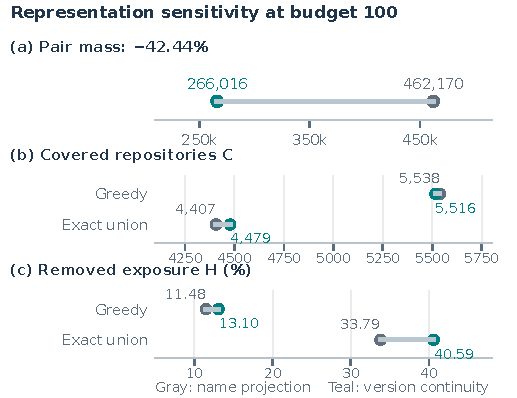
\includegraphics[width=\columnwidth]{representation_detail.pdf}
\caption{Version continuity changes pair mass while aggregate coverage remains similar. The lower panels report coverage and exposure, selecting and evaluating within each representation at budget 100. Both graphs remain observed unions.}
\label{fig:representation}
\end{figure}

Repository deduplication affects decisions. Selecting greedy for all-package coverage, then evaluating repository endpoints, covers 5,308 repositories; selecting for workflow-package coverage gives 5,315. Direct repository selection gives 5,538. Depth ablation gives 5,255 when selection uses portfolio endpoints alone and 5,488 with one-hop evidence, both evaluated against full reach. Endpoint units and depth therefore matter with the final evaluation denominator held fixed.
